%\section{Einleitung}
\subsection{Interceptor}
\begin{frame}
  \frametitle{Interceptor}
  \framesubtitle{Idee}
  \begin{itemize}
    \item Steuert Kommunikation zwischen Komponenten
    \item Eingehende und ausgehende Nachrichten werden abgefangen
    \item Möglicher Einsatz: Sicherheitsüberprüfungen, Protokollierung, Leistungsüberwachung und/oder Fehlerbehebung
  \end{itemize}
\end{frame}

\begin{frame}
  \frametitle{Interceptor}
  \framesubtitle{Pattern}
  \begin{figure}[!ht]
    \centering
    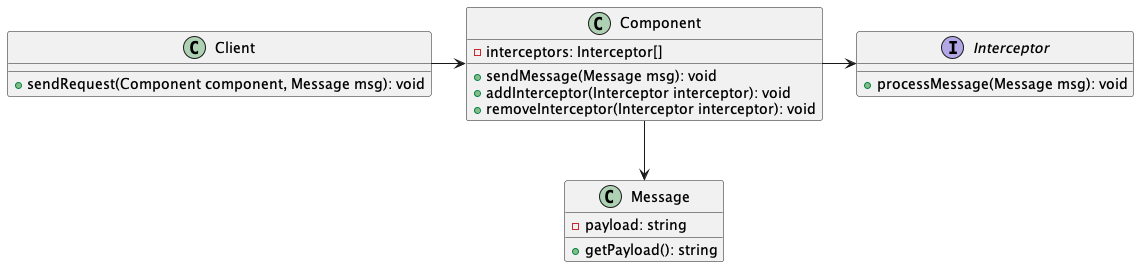
\includegraphics[width=0.99\textwidth]{fig/uml/intercept-class.png}
    \caption{Interceptor Pattern}
    \label{fig:intercept-class}
  \end{figure}
\end{frame}

\begin{frame}
  \frametitle{Interceptor}
  \framesubtitle{Sequenz}
  \begin{figure}[!ht]
    \centering
    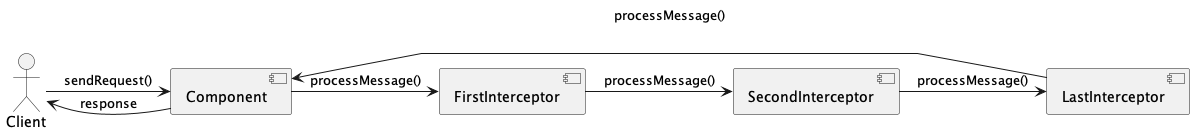
\includegraphics[width=0.99\textwidth]{fig/uml/intercept-seq.png}
    \caption{Interceptor Pattern Sequenz}
    \label{fig:intercept-seq}
  \end{figure}
\end{frame}